\documentclass[12pt]{article}
\usepackage[final]{graphicx}
\usepackage{rotating}
\usepackage{setspace}
\usepackage{amsmath}
\usepackage{amssymb}
\usepackage{amsthm}
\usepackage{subcaption}
\usepackage{breqn}
\usepackage{optidef}
\usepackage{bbm}
\usepackage[utf8]{inputenc}
\usepackage[style=authoryear, backend=biber]{biblatex}
\addbibresource{blinder_weiss_project_bib.bib}
\doublespacing

\title{Solving and estimating \textcite{blinder_weiss_1976_lifecycle_human_capital_labor_supply_synthesis}}
\author{Churn Ken Lee}
\date{}
\begin{document}
\maketitle

\section{Introduction}
I want to estimate a model of lifecycle human capital investment and lifetime labor supply. To do so, I numerically solve the model in \textcite{blinder_weiss_1976_lifecycle_human_capital_labor_supply_synthesis}, and then estimate the model using time use and labor market data.

The model has several unique features: it endogenously generates a period of schooling at the beginning of life, followed by a working period with declining training on the job and a hump-shaped profile of labor supply, and then a period of retirement.

I aim to use this model to match several empirical facts: labor force participation has declined more for lower skilled men compared to higher skilled men, the hours of work of low skilled men has declined relatively more as well (\textcite{aguair_bils_charles_hurst_2017_WP_video_games_labor_supply}), the gap in retirement age between high and low skilled workers has widened (\textcite{rutledge_2018_retirement_age_gap_education}), and the experience-income profile of low skilled workers has flattened more over time (\textcite{elsby_shapiro_2012_AER_trend_growth_employment}).

\begin{figure}[]
    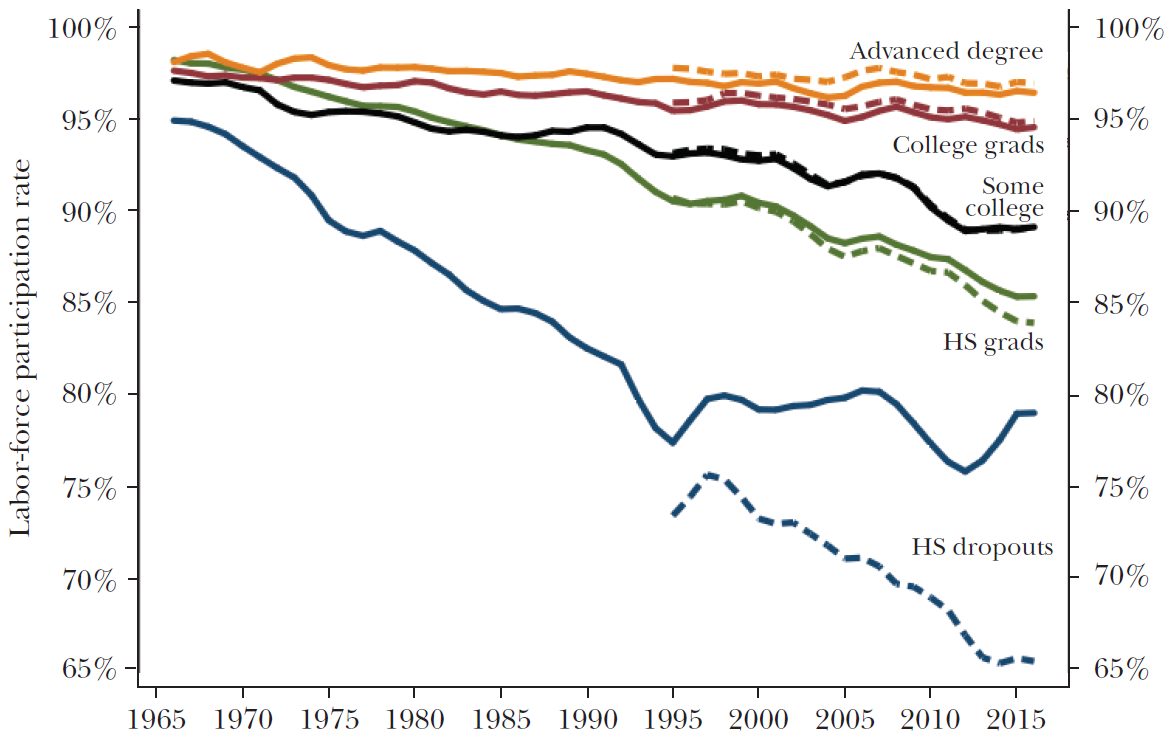
\includegraphics[width = \textwidth]{../../output/participation_education.png}
    \centering
    \caption{Declining LFP of American men, from \textcite{binder_bound_2019_JEP_declining_LFP_less_educated}}
\end{figure}

\begin{figure}[]
    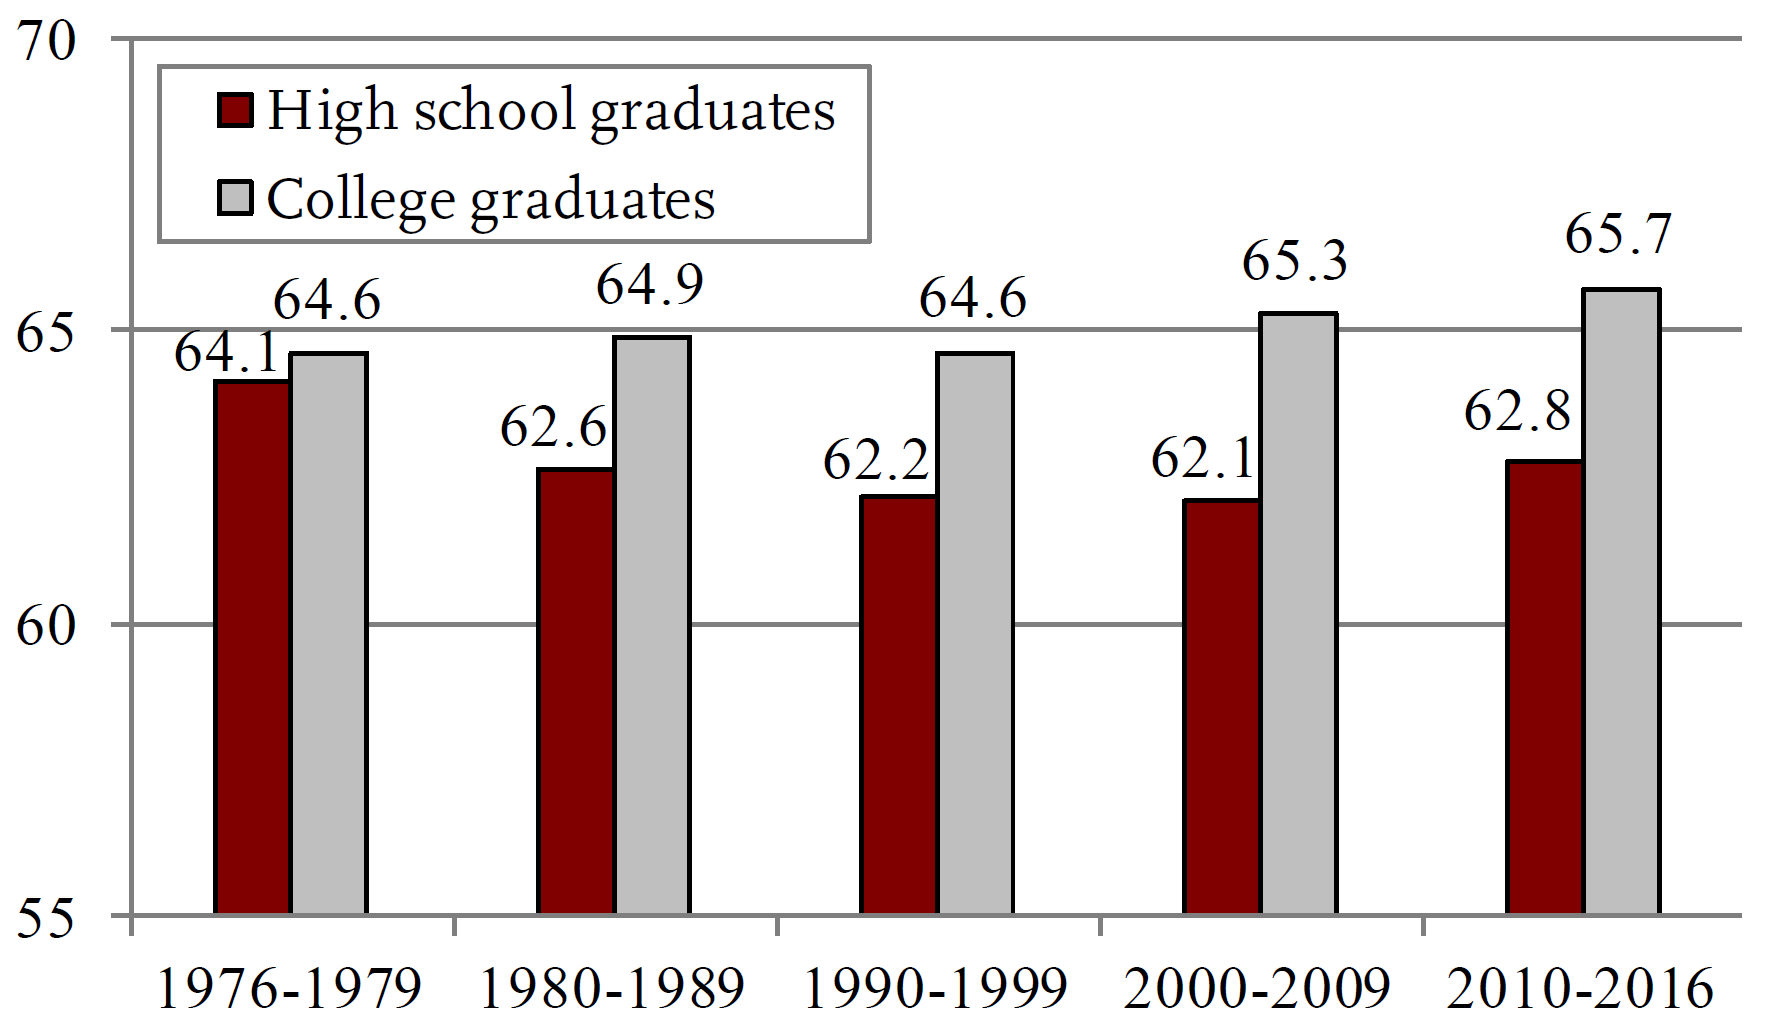
\includegraphics[width = \textwidth]{../../output/retirement.png}
    \centering
    \caption{Increasing retirement age gap, from \textcite{rutledge_2018_retirement_age_gap_education}}
\end{figure}

\begin{figure}[]
    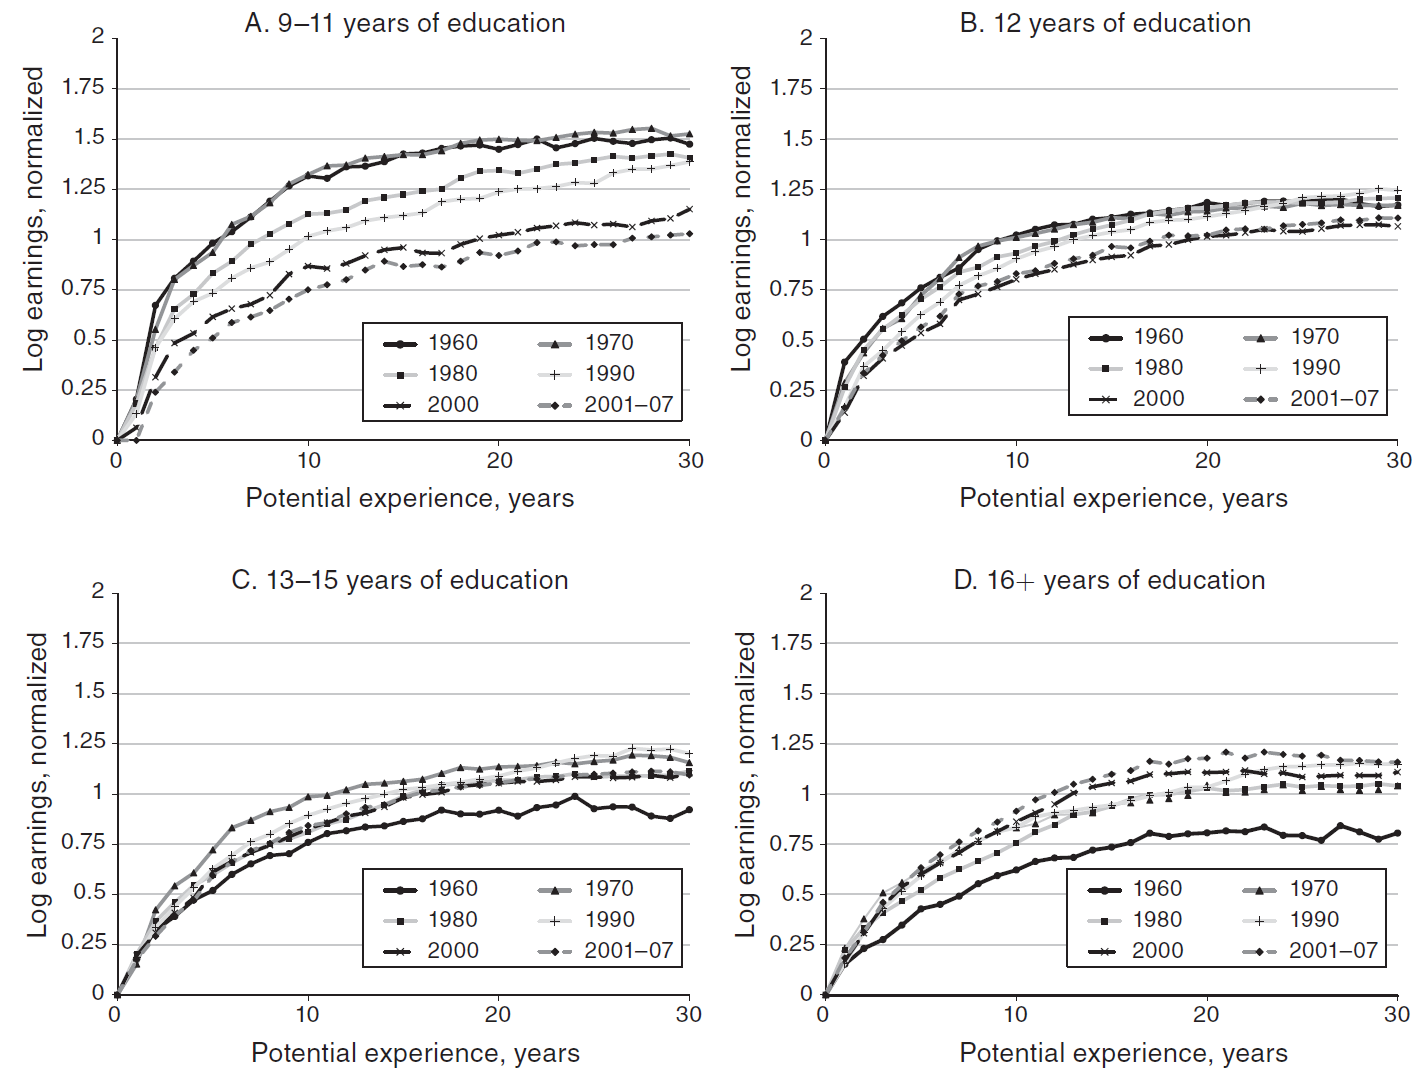
\includegraphics[width = \textwidth]{../../output/profile_cross_elsby_shapiro.png}
    \centering
    \caption{Experience-income profiles have flattened more for low-skilled workers, from \textcite{elsby_shapiro_2012_AER_trend_growth_employment}}
\end{figure}

The canonical model of lifecycle human capital accumulation is the \textcite{ben-porath_1976_human_capital_lifecycle_earnings} model, and is used to explain patterns in wage growth over the lifecycle. 
Some of the earliest empirical estimates of the model are \textcite{heckman_1976_estimate_human_capital_production_function}, \textcite{heckman_1976_lifecycle_human_capital_labor_supply}, \textcite{haley_1976_lifecycle_human_capital}, and \textcite{rosen_1976_lifecycle_human_capital}.
\textcite{browning_hansen_heckman_1999_micro_data_ge_models} reviews this body of earlier work.
These papers typically did not extend the model to include labor supply decisions, with the notable exception of \textcite{heckman_1976_estimate_human_capital_production_function} and \textcite{heckman_1976_lifecycle_human_capital_labor_supply}.
However, even these do not try to model education or retirement decisions explicitly.

Human capital accumulation can also be modelled as a process arising from learning-by-doing. 
In these models, accumulation of human capital occurs exogenously, but only when agents are working.
\textcite{shaw_1989_lifecycle_labor_supply_human_capital} is one of the first papers to empirically estimate such a model.
She also incorporates a labor supply decision, but does not endogenize education or retirement.
More recent work by \textcite{imai_keane_2004_lifecycle_labor_supply_human_capital_accumulation} and \textcite{blundell_costa-dias_meghir_shaw_2016_female_lifecycle_labor_supply_education_human_capital_welfare} endogenizes labor supply decisions, and the latter allows for discrete choices for education levels, but neither allow for endogenous retirement decisions.

On the other hand, lifecycle labor supply models typically treat wages as exogenous when modelling the changes in hours worked over the lifecycle, including retirement.
\textcite{rosen_1976_lifecycle_human_capital} model retirement decisions as arising from non-convexities in choice sets, while \textcite{prescott_rogerson_wallenius_2009_lifetime_aggregate_labor_supply_workweek_length_fixed_costs} uses fixed costs of employment.
Many others explain features of late-in-life labor supply and retirement decisions as arising from features of social insurance programs (\textcite{rush_phelan_1997_labor_supply_incomplete_markets_social_security_medicare}, \textcite{french_2005_retirement_social_security}, \textcite{french_jones_2011_retirement_health_insurance_medicare_social_security}), or complementarities in spousal preferences for leisure (\textcite{casanova_2010_retirement_spouse}).

There is not a lot of work trying to unify the two approaches.
As previously mentioned, \textcite{heckman_1976_lifecycle_human_capital_labor_supply} and \textcite{heckman_1976_estimate_human_capital_production_function} extend the Ben-Porath model to include labor supply decisions, but do not include education or retirement.
\textcite{fan_seshadri_taber_2012_lifetime_labor_supply_human_capital} and \textcite{manuelli_seshadri_shin_2012_lifetime_labor_supply_human_capital} extend the Ben-Porath model to include indivisible labor supply and retirement, but does not include endogenous education choice.

The \textcite{blinder_weiss_1976_lifecycle_human_capital_labor_supply_synthesis} has many desirable features in this regard.
It extends the Ben-Porath approach by endogenizing education, labor supply, and retirement decisions.
The drawback is that allowing for continuous labor supply and human capital accumulation decisions is incredibly computationally demanding, as discussed in \textcite{imai_keane_2004_lifecycle_labor_supply_human_capital_accumulation}.

\iffalse
\section{Organize my thoughts}
\subsection{Lifecycle human capital models}
\begin{itemize}
    \item \textcite{ben-porath_1976_human_capital_lifecycle_earnings}: canonical model, does not have labor supply decisions
    \item \textcite{kuruscu_2006_lifecycle_training}
    \item Early estimates of Ben-Porath: \textcite{rosen_1976_lifecycle_human_capital} and \textcite{haley_1976_lifecycle_human_capital}
    \item Early empirical work reviewed in \textcite{browning_hansen_heckman_1999_micro_data_ge_models}
    \item More recent estimate: \textcite{kuruscu_2006_lifecycle_training}
\end{itemize}

\subsection{Lifetime labor supply models}
\begin{itemize}
    \item Retirement literature assumes exogenous wage processes
    \item \textcite{rogerson_wallenius_2013_retirement_nonconvexities}: Nonconvex choice sets
    \item 
\end{itemize}

\subsection{Combination}
\begin{itemize}
    \item Ben-Porath + labor supply: \textcite{heckman_1976_lifecycle_human_capital_labor_supply} and \textcite{heckman_1976_estimate_human_capital_production_function} do not contain endogenous education or retirement decisions
    \item \textcite{imai_keane_2004_lifecycle_labor_supply_human_capital_accumulation}: Learning-by-doing + lifecycle labor supply; does not have endogenous education or retirement
    \item \textcite{keane_wolpin_1997_career_decisions_young_men}: Education (sort of), retirement, lifecycle labor supply, learning-by-doing: all discrete choices
    \item \textcite{blundell_costa-dias_meghir_shaw_2016_female_lifecycle_labor_supply_education_human_capital_welfare}: Lifecycle labor supply + learning-by-doing, Discrete education choice, no retirement choice
    \item Ben-Porath + labor supply: \textcite{manuelli_seshadri_shin_2012_lifetime_labor_supply_human_capital} and \textcite{fan_seshadri_taber_2012_lifetime_labor_supply_human_capital}, indivisible labor supply, no endogenous education choice
    \item \textcite{shaw_1989_lifecycle_labor_supply_human_capital}: Learning-by-doing + lifecycle labor supply, first to estimate LBD model, no endogenous education or retirement
\end{itemize}

Key advantage of \textcite{blinder_weiss_1976_lifecycle_human_capital_labor_supply_synthesis}: It integrates many of these features in one model.

\subsection{Motivation}
\begin{itemize}
    \item Declining experience-wage profile for low-skilled relative to high-skilled
    \item Selection means decline was actually larger?
    \item Decrease in work-hours of low-skilled relative to high-skilled
    \item Increase in retirement age gap
    \item Decline in LFP among low-skilled relative to high-skilled
    \item Non-participation among low-skilled and in-and-outs? In-and-outs are not increasing investment in human capital; most time goes to increased leisure
    \item Reversal of flattening in recent years
    \item Income, not wages
    \item Blinder and Weiss generates experience-wage (and income) profile
\end{itemize}

\fi

\section{Lifecycle model of human capital accumulation and labor supply in \textcite{blinder_weiss_1976_lifecycle_human_capital_labor_supply_synthesis}}
Agents have finite lifespan $T$, and they derive utility from a stream of consumption, $c(t)$, leisure $1 - h(t)$, and a bequest of their terminal asset holdings $A(T)$.
They own two assets: savings $A(t)$ and human capital $K(t)$.
They earn a rate of return $r$ on savings, and human capital depreciates at rate $\delta$.
They have a constant discount rate $\rho$, and so have lifetime utility
\begin{equation}
    \int_{t = 0}^{T} e^{-\rho t} u(c(t), 1-h(t)) dt + B(A(t))
\end{equation}

They choose consumption $c_(t)$, labor supply $h(t)$, and human capital investment choice $x(t)$ to maximize lifetime utility, subject to the evolution of savings,
\begin{equation}
    \dot{A} = r A + h g(x) K - c,
\end{equation}
human capital,
\begin{equation}
    \dot{K} = -\delta K + x h K,
\end{equation}
period time constraint
\begin{equation}
    l_t \in [0,1],
\end{equation}
and initial conditions $A(0), K(0)$.

The function $g(x)$ governs the tradeoff between accumulating human capital and financial compensation from supplying labor. 
We can interpret it as a reduced form representation of equilibrium labor market outcomes.
This is similar to one interpretation of the training vs earning choice in \textcite{ben-porath_1976_human_capital_lifecycle_earnings}, whereby jobs that provide more training pay lower wages.
One difference is that here the concavity is in the tradeoff and the production function for human capital is linear, while in \textcite{ben-porath_1976_human_capital_lifecycle_earnings} the tradeoff is linear and the production function is concave.

The function $g(\cdot)$ has to satisfy several properties:
\begin{enumerate}
    \item $g(\cdot)$ is a concave, continuous, and decreasing function over the interval $[0,1]$ \label{labor_market_eqm}
    \item $g'(0) < 0$ and $g'(1) > -\infty$ \label{g_corners}
    \item $g(0) = 1$ and $g(1) = 0$ \label{normalization}
\end{enumerate}
Property \ref{g_corners} allows for the existence of corners $x_t = 0$ and $x_t = 1$ in the optimal path.
For example, if $g'(0) = 0$, then no agent would choose $x = 0$ as a slightly higher $x$ would entail no decrease in wages but a positive amount of human capital accumulation. 
The possibility of these corners is key to the model. If agents are sufficiently patient, they choose $x = 1$ in the early periods of their lives, which is interpreted as schooling.
They will also choose $l = 1$ for the last periods of their lives, which is interpreted as retirement.
Property \ref{normalization} allows for interpreting $g(x)$ as the proportion of potential earnings capacity, $K$, that is realized with the choice of $x$.

If $\rho < r + \delta$, i.e., agents are sufficiently patient, then the model endogenously generates four succeeding periods of life:
\begin{itemize}
    \item Period 1: $h > 0$, $x = 1$ (schooling)
    \item Period 2: $h > 0$, $0 < x < 1$ (on-the-job training)
    \item Period 3: $h > 0$, $x = 0$ (pure work)
    \item Period 4: $h = 0$ (retirement)
\end{itemize}
These have features that I want to empirically match trends I see in the data.

\section{Solution strategies}
I am trying two different approaches in parallel: shooting method, and a finite-difference approximation to the HJB equation using an upwind scheme.

\subsection{Shooting Method}
As laid out in \textcite{blinder_weiss_1976_lifecycle_human_capital_labor_supply_synthesis}, the Hamiltonian for the household's optimization problem is
\begin{equation}
    H(c, h, x, A, K, \mu, p) = e^{-\rho t} \left\{ u(c, 1-h) + p K (axh - \delta) + \mu \left[ rA + g(x) h K - c \right] \right\}
\end{equation}
Pontryagin's maximum principle implies the following set of first order conditions:
\begin{align}
    U_{c}(c, l) =\mu \\
    U_{l}(c, l) =\mu K g(x)+a p K x \quad &\text { if } \quad 0<l<1 \\
    U_{l}(c, l) \geq \mu K g(x)+a p K x \quad &\text { if } l=1 \\
    h\left[a p K+\mu K g^{\prime}(x)\right]=0 \quad &\text { if } \quad 0<x<1 \\
    h\left[a p K+\mu K g^{\prime}(0)\right] \leq 0 \quad &\text { if } \quad x=0 \\
    h\left[a p K+\mu K g^{\prime}(1)\right] \geq 0 \quad &\text { if } x=1 \\
    \dot{\mu} / \mu=\rho-r & \\
    \dot{p} / p=\rho+\delta-a x h-g(x) h \mu / p
\end{align}
where $\mu$ and $p$ are the shadow prices of $A$ and $K$ respectively. 
The terminal conditions are $K(T)p(T) = 0$ and $\mu(T) = B'(A(T))$.
For any given state $K$ and $A$, these equations pin down $c, h, x$ (and thus the evolution of $K$ and $A$), and the evolution of $\mu$ and $p$, given starting values of $\mu$ and $p$.

Hence, for initial values of $K$ and $A$, one can guess starting values of $\mu$ and $p$ that will lead to the system to terminate with values that satisfy the terminal conditions.

This method can produce sensible solutions, but the method is sensitive to the choice of initial values of $K$, $A$, and parameter values.
One example is given in figure \ref{fig:shooting_solution}.
However, for most values I have tried, the solutions are completely nonsensical.


\begin{figure}[h]
    \begin{subfigure}{.5\textwidth}
      \centering
      % include first image
      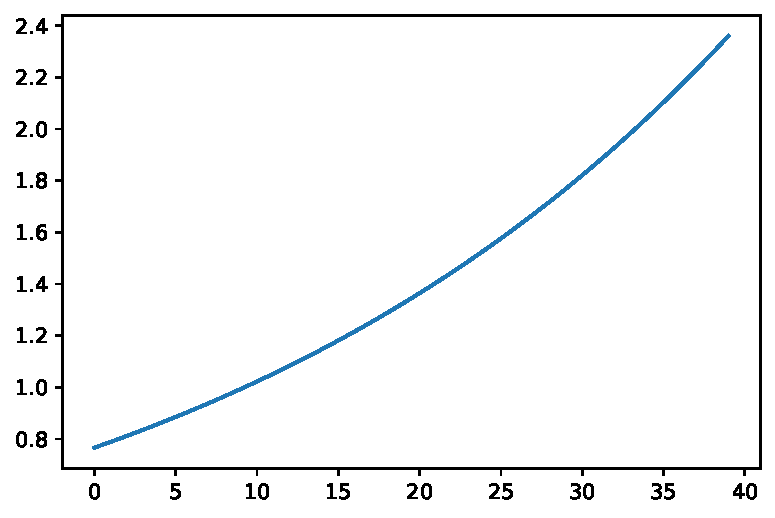
\includegraphics[width=.8\linewidth]{../../output/shooting_c_path.pdf}  
      \caption{Path of $c$}
      \label{fig:c_path}
    \end{subfigure}
    \begin{subfigure}{.5\textwidth}
      \centering
      % include second image
      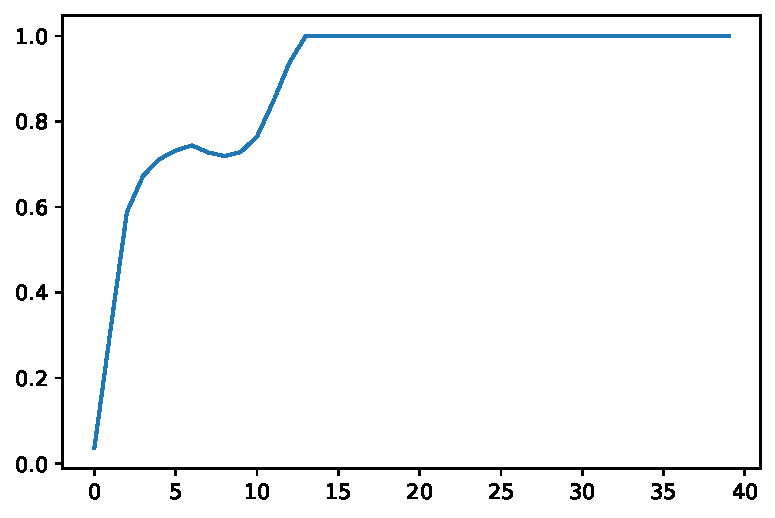
\includegraphics[width=.8\linewidth]{../../output/shooting_l_path.pdf}  
      \caption{Path of $l$}
      \label{fig:l_path}
    \end{subfigure}
    
    \begin{subfigure}{.5\textwidth}
      \centering
      % include third image
      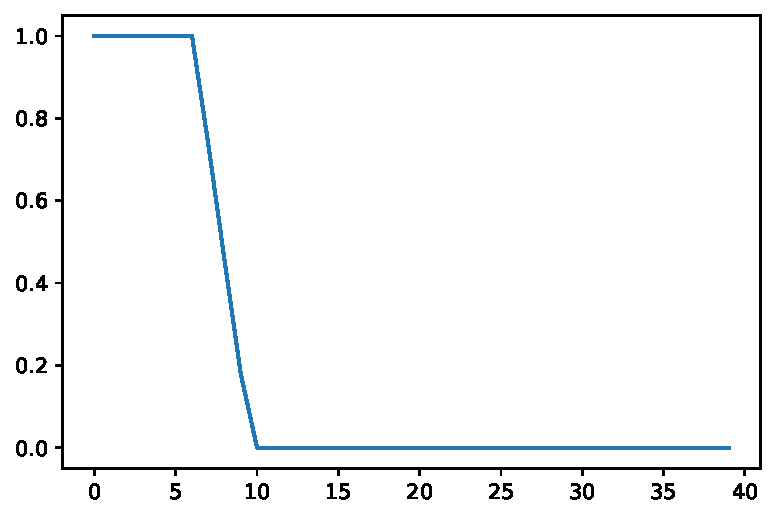
\includegraphics[width=.8\linewidth]{../../output/shooting_x_path.pdf}  
      \caption{Path of $x$}
      \label{fig:x_path}
    \end{subfigure}
    \begin{subfigure}{.5\textwidth}
      \centering
      % include fourth image
      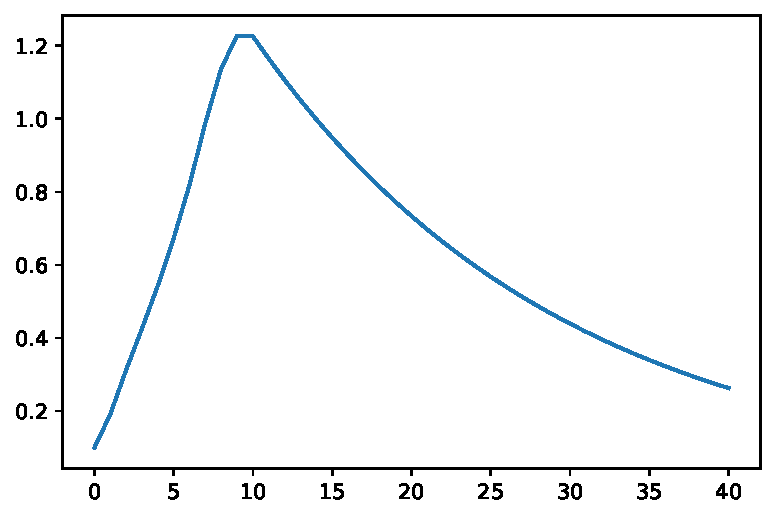
\includegraphics[width=.8\linewidth]{../../output/shooting_K_path.pdf}  
      \caption{Path of $K$}
      \label{fig:h_path}
    \end{subfigure}

    \begin{subfigure}{.5\textwidth}
        \centering
        % include fifth image
        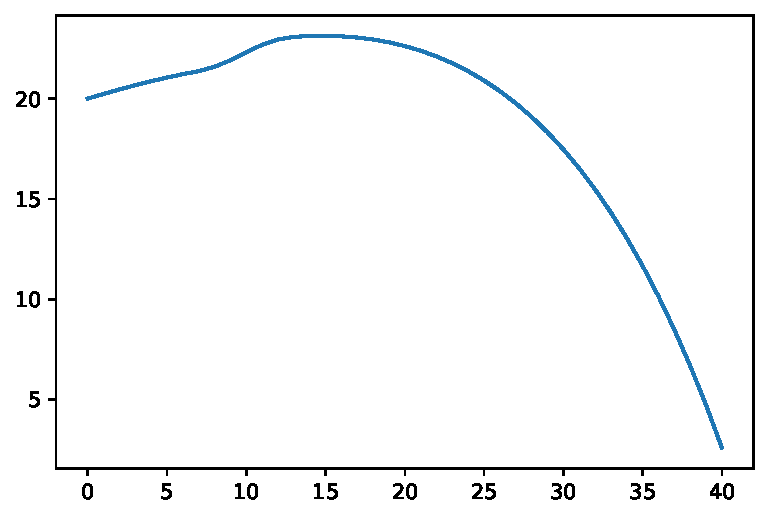
\includegraphics[width=.8\linewidth]{../../output/shooting_A_path.pdf}  
        \caption{Path of $A$}
        \label{fig:x_path}
    \end{subfigure}
    \caption{An example of a solution obtained using the shooting method.}
    \label{fig:shooting_solution}
\end{figure}

\subsection{Finite difference approximation + upwind scheme}
The solution strategy I am focusing most of my efforts on is mostly based on Ben Moll's notes on using finite difference methods with an upwind scheme to solve macroeconomic models.

The HJB equation for the agent's problem is
\begin{align*}
    \rho V(A, K, t) = \max_{c, h, x} \quad &u(c, 1-h) \\
    &+ \partial_A V(A, K, t) \left[rA + h g(x) K - c \right] \\
    &+ \partial_K V(A, K, t) \left[-\delta K + x h K \right] \\
    &+ \partial_t V(A, K, t)
\end{align*}
which will be solved by approximating the value function and its partial derivatives using a finite difference upwind scheme.
I approximate $V(A, K, t)$ on $nA*nK$ discrete points in the state space, where $nA$ and $nK$ are the number of grid points for $A$ and $K$ respectively.
Denote the index for $A$ and $K$ as $i$ and $j$ respectively, and denote $V(A_i, K_j, t) = V_{ij}^t$.
At point $A_i, K_j, t$, I can approximate the partial derivatives using forward difference:
\begin{align}
    \partial_A^F V_{i,j}^t &= \frac{V_{i+1, j}^t - V_{i, j}^t}{\Delta A}, \\
    \partial_K^F V_{i,j}^t &= \frac{V_{i, j+1}^t - V_{i, j}^t}{\Delta A},
\end{align}
or backward difference:
\begin{align}
    \partial_A^B V_{i,j}^t &= \frac{V_{i, j}^t - V_{i-1, j}^t}{\Delta A}, \\
    \partial_K^B V_{i,j}^t &= \frac{V_{i, j}^t - V_{i, j-1}^t}{\Delta A},
\end{align}
Forward difference is used if the drift of the state variable is positive, and backwards difference is used if the drift is negative.
The drift is determined using the first order conditions:
\begin{align}
    \partial_c u(c_{i,j}^t, h_{i,j}^t) &= \partial_A V_{i,j}^t \\
    \partial_h u(c_{i,j}^t, h_{i,j}^t) &= \partial_A V_{i,j}^t \left[ g(x_{i, j}^t) K \right] + \partial_K V_{i,j}^t \left[ x_{i, j}^t K \right] \\
    0 &= \partial_A V_{i,j}^t \left[ h g'(x_{i, j}^t) K \right] + \partial_K V_{i,j}^t \left[ h K \right]
\end{align}
together with constraints $0 \leq h \leq 1$, $0 \leq x \leq 1$.

For a given approximation scheme, e.g., $FB$ (forward difference for $A$, backwards difference for $K$), the FOCs produce optimal $c_{i,j}^t, h_{i,j}^t, x_{i,j}^t$.
These can then be used to compute drifts for $A$ and $K$: $\mu_{A, i,j}^{FB}$ and $\mu_{K, i,j}^{FB}$.
If these drifts are consistent with the approximation scheme, i.e., $\mu_{A, i,j}^{FB} > 0, \mu_{K, i,j}^{FB} < 0$, then the $FB$ scheme will be used to approximate $\partial V_{ij}^t$.
The HJB can then be discretized as
\begin{align}
    \rho V_{i,j}^t = u(c_{i,j}^t, 1-h_{i,j}^t) + \partial_A^F V_{i,j}^t \left[ \mu_{A: i, j}^{FF} \mathbbm{1}_{A: i, j}^{FF} + \mu_{A: i, j}^{FB} \mathbbm{1}_{A: i, j}^{FB} \right] \label{discretized_HJB} \\
    + \partial_A^B V_{i,j}^t \left[ \mu_{A: i, j}^{BF} \mathbbm{1}_{A: i, j}^{BF} + \mu_{A: i, j}^{BB} \mathbbm{1}_{A: i, j}^{BB} \right] \nonumber \\
    + \partial_K^F V_{i,j}^t \left[ \mu_{K: i, j}^{FF} \mathbbm{1}_{K: i, j}^{FF} + \mu_{K: i, j}^{BF} \mathbbm{1}_{K: i, j}^{BF} \right] \nonumber\\
    + \partial_K^B V_{i,j}^t \left[ \mu_{K: i, j}^{FB} \mathbbm{1}_{K: i, j}^{FB} + \mu_{K: i, j}^{BB} \mathbbm{1}_{K: i, j}^{BB} \right] \nonumber \\
    + \frac{V_{i,j}^{t+1} - V_{i,j}^{t}}{\Delta t} \nonumber
\end{align}
where $\mathbbm{1}_{A:i,j}^{FF}$ is an indicator function for the consistency of the $FF$ scheme for $A$.

The value function for all the grid points $i, j$ at period $t$ can be stacked into a single vector, $V^t$, and the discretized HJB can be compactly written as
\begin{equation}
    \rho V^t = u(V^{t+1}) + A(V^{t+1}) V^t + \frac{V^{t+1} - V^t}{\Delta t} \label{HJB_stacked}
\end{equation}
where $A(V^{t+1})$ is an ($na*nk$) by ($na*nk$) square diagonal sparse matrix that contains the terms in the square brackets in (\ref{discretized_HJB}) in appropriate positions.

Together with terminal conditions
\begin{equation}
    V^T_{i,j} = B(A_{i,j}),
\end{equation}
I can solve (\ref{HJB_stacked}) backwards from $T$.

I am currently trying to code up this solution method, but I am running into a few difficulties, e.g., the non-invertibility of $A$. I intend to continue working on this through the summer.

\printbibliography
\end{document}